\documentclass[twocolumn]{IEEEtran}  % peerreviewca,draftcls

\usepackage{xcolor}
\newcommand{\note}[1]{\textcolor{red}{\textbf{#1}}}

% Some very useful LaTeX packages include:
% (uncomment the ones you want to load)


% *** MISC UTILITY PACKAGES ***
%
%\usepackage{ifpdf}
% Heiko Oberdiek's ifpdf.sty is very useful if you need conditional
% compilation based on whether the output is pdf or dvi.
% usage:
% \ifpdf
%   % pdf code
% \else
%   % dvi code
% \fi
% The latest version of ifpdf.sty can be obtained from:
% http://www.ctan.org/pkg/ifpdf
% Also, note that IEEEtran.cls V1.7 and later provides a builtin
% \ifCLASSINFOpdf conditional that works the same way.
% When switching from latex to pdflatex and vice-versa, the compiler may
% have to be run twice to clear warning/error messages.






% *** CITATION PACKAGES ***
%
%\usepackage{cite}
% cite.sty was written by Donald Arseneau
% V1.6 and later of IEEEtran pre-defines the format of the cite.sty package
% \cite{} output to follow that of the IEEE. Loading the cite package will
% result in citation numbers being automatically sorted and properly
% "compressed/ranged". e.g., [1], [9], [2], [7], [5], [6] without using
% cite.sty will become [1], [2], [5]--[7], [9] using cite.sty. cite.sty's
% \cite will automatically add leading space, if needed. Use cite.sty's
% noadjust option (cite.sty V3.8 and later) if you want to turn this off
% such as if a citation ever needs to be enclosed in parenthesis.
% cite.sty is already installed on most LaTeX systems. Be sure and use
% version 5.0 (2009-03-20) and later if using hyperref.sty.
% The latest version can be obtained at:
% http://www.ctan.org/pkg/cite
% The documentation is contained in the cite.sty file itself.






% *** GRAPHICS RELATED PACKAGES ***
%
\ifCLASSINFOpdf
  \usepackage[pdftex]{graphicx}
  % declare the path(s) where your graphic files are
  \graphicspath{{figures/}}
  % and their extensions so you won't have to specify these with
  % every instance of \includegraphics
  \DeclareGraphicsExtensions{.pdf,.jpeg,.png}
\else
  % or other class option (dvipsone, dvipdf, if not using dvips). graphicx
  % will default to the driver specified in the system graphics.cfg if no
  % driver is specified.
  \usepackage[dvips]{graphicx}
  % declare the path(s) where your graphic files are
  \graphicspath{{figures/}}
  % and their extensions so you won't have to specify these with
  % every instance of \includegraphics
  \DeclareGraphicsExtensions{.eps}
\fi
% graphicx was written by David Carlisle and Sebastian Rahtz. It is
% required if you want graphics, photos, etc. graphicx.sty is already
% installed on most LaTeX systems. The latest version and documentation
% can be obtained at: 
% http://www.ctan.org/pkg/graphicx
% Another good source of documentation is "Using Imported Graphics in
% LaTeX2e" by Keith Reckdahl which can be found at:
% http://www.ctan.org/pkg/epslatex
%
% latex, and pdflatex in dvi mode, support graphics in encapsulated
% postscript (.eps) format. pdflatex in pdf mode supports graphics
% in .pdf, .jpeg, .png and .mps (metapost) formats. Users should ensure
% that all non-photo figures use a vector format (.eps, .pdf, .mps) and
% not a bitmapped formats (.jpeg, .png). The IEEE frowns on bitmapped formats
% which can result in "jaggedy"/blurry rendering of lines and letters as
% well as large increases in file sizes.
%
% You can find documentation about the pdfTeX application at:
% http://www.tug.org/applications/pdftex

\usepackage{tikz}
\usepackage{pgfplots} 
\pgfplotsset{compat=newest} 
\pgfplotsset{plot coordinates/math parser=false}
\newlength\fwidth
\newlength\hwidth



% *** MATH PACKAGES ***
%
\usepackage{amsmath}
\usepackage{amsfonts}
% A popular package from the American Mathematical Society that provides
% many useful and powerful commands for dealing with mathematics.
%
% Note that the amsmath package sets \interdisplaylinepenalty to 10000
% thus preventing page breaks from occurring within multiline equations. Use:
%\interdisplaylinepenalty=2500
% after loading amsmath to restore such page breaks as IEEEtran.cls normally
% does. amsmath.sty is already installed on most LaTeX systems. The latest
% version and documentation can be obtained at:
% http://www.ctan.org/pkg/amsmath





% *** SPECIALIZED LIST PACKAGES ***
%
% \usepackage{algorithmic}
\usepackage{algorithm,algpseudocode}

% make algo small
\makeatletter
\renewcommand{\ALG@beginalgorithmic}{\small}
\makeatother

% algorithmic.sty was written by Peter Williams and Rogerio Brito.
% This package provides an algorithmic environment fo describing algorithms.
% You can use the algorithmic environment in-text or within a figure
% environment to provide for a floating algorithm. Do NOT use the algorithm
% floating environment provided by algorithm.sty (by the same authors) or
% algorithm2e.sty (by Christophe Fiorio) as the IEEE does not use dedicated
% algorithm float types and packages that provide these will not provide
% correct IEEE style captions. The latest version and documentation of
% algorithmic.sty can be obtained at:
% http://www.ctan.org/pkg/algorithms
% Also of interest may be the (relatively newer and more customizable)
% algorithmicx.sty package by Szasz Janos:
% http://www.ctan.org/pkg/algorithmicx


% *** ALIGNMENT PACKAGES ***
%
%\usepackage{array}
% Frank Mittelbach's and David Carlisle's array.sty patches and improves
% the standard LaTeX2e array and tabular environments to provide better
% appearance and additional user controls. As the default LaTeX2e table
% generation code is lacking to the point of almost being broken with
% respect to the quality of the end results, all users are strongly
% advised to use an enhanced (at the very least that provided by array.sty)
% set of table tools. array.sty is already installed on most systems. The
% latest version and documentation can be obtained at:
% http://www.ctan.org/pkg/array


% IEEEtran contains the IEEEeqnarray family of commands that can be used to
% generate multiline equations as well as matrices, tables, etc., of high
% quality.




% *** SUBFIGURE PACKAGES ***
%\ifCLASSOPTIONcompsoc
%  \usepackage[caption=false,font=normalsize,labelfont=sf,textfont=sf]{subfig}
%\else
%  \usepackage[caption=false,font=footnotesize]{subfig}
%\fi
% subfig.sty, written by Steven Douglas Cochran, is the modern replacement
% for subfigure.sty, the latter of which is no longer maintained and is
% incompatible with some LaTeX packages including fixltx2e. However,
% subfig.sty requires and automatically loads Axel Sommerfeldt's caption.sty
% which will override IEEEtran.cls' handling of captions and this will result
% in non-IEEE style figure/table captions. To prevent this problem, be sure
% and invoke subfig.sty's "caption=false" package option (available since
% subfig.sty version 1.3, 2005/06/28) as this is will preserve IEEEtran.cls
% handling of captions.
% Note that the Computer Society format requires a larger sans serif font
% than the serif footnote size font used in traditional IEEE formatting
% and thus the need to invoke different subfig.sty package options depending
% on whether compsoc mode has been enabled.
%
% The latest version and documentation of subfig.sty can be obtained at:
% http://www.ctan.org/pkg/subfig




% *** FLOAT PACKAGES ***
%
%\usepackage{fixltx2e}
% fixltx2e, the successor to the earlier fix2col.sty, was written by
% Frank Mittelbach and David Carlisle. This package corrects a few problems
% in the LaTeX2e kernel, the most notable of which is that in current
% LaTeX2e releases, the ordering of single and double column floats is not
% guaranteed to be preserved. Thus, an unpatched LaTeX2e can allow a
% single column figure to be placed prior to an earlier double column
% figure.
% Be aware that LaTeX2e kernels dated 2015 and later have fixltx2e.sty's
% corrections already built into the system in which case a warning will
% be issued if an attempt is made to load fixltx2e.sty as it is no longer
% needed.
% The latest version and documentation can be found at:
% http://www.ctan.org/pkg/fixltx2e


%\usepackage{stfloats}
% stfloats.sty was written by Sigitas Tolusis. This package gives LaTeX2e
% the ability to do double column floats at the bottom of the page as well
% as the top. (e.g., "\begin{figure*}[!b]" is not normally possible in
% LaTeX2e). It also provides a command:
%\fnbelowfloat
% to enable the placement of footnotes below bottom floats (the standard
% LaTeX2e kernel puts them above bottom floats). This is an invasive package
% which rewrites many portions of the LaTeX2e float routines. It may not work
% with other packages that modify the LaTeX2e float routines. The latest
% version and documentation can be obtained at:
% http://www.ctan.org/pkg/stfloats
% Do not use the stfloats baselinefloat ability as the IEEE does not allow
% \baselineskip to stretch. Authors submitting work to the IEEE should note
% that the IEEE rarely uses double column equations and that authors should try
% to avoid such use. Do not be tempted to use the cuted.sty or midfloat.sty
% packages (also by Sigitas Tolusis) as the IEEE does not format its papers in
% such ways.
% Do not attempt to use stfloats with fixltx2e as they are incompatible.
% Instead, use Morten Hogholm'a dblfloatfix which combines the features
% of both fixltx2e and stfloats:
%
% \usepackage{dblfloatfix}
% The latest version can be found at:
% http://www.ctan.org/pkg/dblfloatfix




%\ifCLASSOPTIONcaptionsoff
%  \usepackage[nomarkers]{endfloat}
% \let\MYoriglatexcaption\caption
% \renewcommand{\caption}[2][\relax]{\MYoriglatexcaption[#2]{#2}}
%\fi
% endfloat.sty was written by James Darrell McCauley, Jeff Goldberg and 
% Axel Sommerfeldt. This package may be useful when used in conjunction with 
% IEEEtran.cls'  captionsoff option. Some IEEE journals/societies require that
% submissions have lists of figures/tables at the end of the paper and that
% figures/tables without any captions are placed on a page by themselves at
% the end of the document. If needed, the draftcls IEEEtran class option or
% \CLASSINPUTbaselinestretch interface can be used to increase the line
% spacing as well. Be sure and use the nomarkers option of endfloat to
% prevent endfloat from "marking" where the figures would have been placed
% in the text. The two hack lines of code above are a slight modification of
% that suggested by in the endfloat docs (section 8.4.1) to ensure that
% the full captions always appear in the list of figures/tables - even if
% the user used the short optional argument of \caption[]{}.
% IEEE papers do not typically make use of \caption[]'s optional argument,
% so this should not be an issue. A similar trick can be used to disable
% captions of packages such as subfig.sty that lack options to turn off
% the subcaptions:
% For subfig.sty:
% \let\MYorigsubfloat\subfloat
% \renewcommand{\subfloat}[2][\relax]{\MYorigsubfloat[]{#2}}
% However, the above trick will not work if both optional arguments of
% the \subfloat command are used. Furthermore, there needs to be a
% description of each subfigure *somewhere* and endfloat does not add
% subfigure captions to its list of figures. Thus, the best approach is to
% avoid the use of subfigure captions (many IEEE journals avoid them anyway)
% and instead reference/explain all the subfigures within the main caption.
% The latest version of endfloat.sty and its documentation can obtained at:
% http://www.ctan.org/pkg/endfloat
%
% The IEEEtran \ifCLASSOPTIONcaptionsoff conditional can also be used
% later in the document, say, to conditionally put the References on a 
% page by themselves.




% *** PDF, URL AND HYPERLINK PACKAGES ***
%
%\usepackage{url}
% url.sty was written by Donald Arseneau. It provides better support for
% handling and breaking URLs. url.sty is already installed on most LaTeX
% systems. The latest version and documentation can be obtained at:
% http://www.ctan.org/pkg/url
% Basically, \url{my_url_here}.




% *** Do not adjust lengths that control margins, column widths, etc. ***
% *** Do not use packages that alter fonts (such as pslatex).         ***
% There should be no need to do such things with IEEEtran.cls V1.6 and later.
% (Unless specifically asked to do so by the journal or conference you plan
% to submit to, of course. )


%%%%%%%%%%%%%%%%% Macros used in the paper %%%%%%%%%%%%%%%%%%%%

\usepackage{xspace}

\newtheorem{definition}{Definition}
\newtheorem{lemma}{Lemma}
\newtheorem{problem}{Problem}
\newtheorem{remark}{Remark}

\newcommand{\GaussianDist}[2]{\ensuremath{\operatorname*{\mathcal{N}}\left(#1, #2\right)}}  % Gaussian distribution given mean and variance
\newcommand{\GaussianDistSmall}[2]{\ensuremath{\operatorname*{\mathcal{N}}(#1, #2)}}  % Gaussian distribution given mean and variance

\newcommand{\st}{\mbox{\text{subject to}}}

\newcommand{\sigmamax}[1][0]{\ensuremath{\overbar{\sigma}_{#1}}}

\newcommand{\eg}{e.g.,\xspace}
\newcommand{\ie}{i.e.,\xspace}
\newcommand{\etc}{etc.\xspace}
\newcommand{\cf}{cf.~}

% Some commonly used math functions/operators
\DeclareMathOperator*{\argmin}{arg\,min}
\DeclareMathOperator*{\argmax}{arg\,max}
\DeclareMathOperator*{\minimize}{minimize}
\DeclareMathOperator*{\maximize}{maximize}
\DeclareMathOperator{\sgn}{sgn}  % the signum/sign function
\DeclareMathOperator*{\cov}{Cov} % covariance
\DeclareMathOperator*{\var}{Var} % variance
\DeclareMathOperator*{\diag}{diag} % diagonal

\newcommand{\RR}{\mathbb{R}\xspace}  % Real set
\newcommand{\NN}{\mathbb{N}\xspace}  % Natural number set
\newcommand{\QQ}{\mathbb{Q}\xspace}  % Rational number set
\newcommand{\CC}{\mathbb{C}\xspace}  % Complex number set
\newcommand{\ZZ}{\mathbb{Z}\xspace}  % Integer number set
\newcommand{\EE}{\mathbb{E}\xspace}  % Expectation
\newcommand{\PP}{\mathbb{P}\xspace}  % Probability
\newcommand{\BB}{\mathbb{B}\xspace}  % Logic set {true, false}
\newcommand{\D}{\mathcal{D}\xspace}
\newcommand{\C}{\mathcal{C}\xspace}


% correct bad hyphenation here
%\hyphenation{op-tical net-works semi-conduc-tor}

\def\papertitle{[Temporary] Learning to Control Smart (Building) Energy Systems (with Gaussian Processes)}

\begin{document}
%
% paper title
% Titles are generally capitalized except for words such as a, an, and, as,
% at, but, by, for, in, nor, of, on, or, the, to and up, which are usually
% not capitalized unless they are the first or last word of the title.
% Linebreaks \\ can be used within to get better formatting as desired.
% Do not put math or special symbols in the title.
\title{\papertitle}
%
%
% author names and IEEE memberships
% note positions of commas and nonbreaking spaces ( ~ ) LaTeX will not break
% a structure at a ~ so this keeps an author's name from being broken across
% two lines.
% use \thanks{} to gain access to the first footnote area
% a separate \thanks must be used for each paragraph as LaTeX2e's \thanks
% was not built to handle multiple paragraphs
%

\author{Truong~X.~Nghiem,~\IEEEmembership{Member,~IEEE,}
        Achin~Jain,~\IEEEmembership{Student Member,~IEEE,}
        and~Rahul~Mangharam,~\IEEEmembership{Member,~IEEE}% <-this % stops a space
        \thanks{T. X. Nghiem is with the School of Informatics, Computing, and Cyber Systems, Northern Arizona University, Flagstaff, AZ 86001, USA; email: \texttt{truong.nghiem@nau.edu}.}% <-this % stops a space
\thanks{A. Jain and R. Mangharam are with the Department of Electrical and Systems Engineering, University of Pennsylvanua, Philadelphia, PA 19104, USA; emails: \texttt{(achinj,rahulm)@seas.upenn.edu}.}}% <-this % stops a space
%\thanks{Manuscript received April 19, 2005; revised August 26, 2015.}}

% note the % following the last \IEEEmembership and also \thanks - 
% these prevent an unwanted space from occurring between the last author name
% and the end of the author line. i.e., if you had this:
% 
% \author{....lastname \thanks{...} \thanks{...} }
%                     ^------------^------------^----Do not want these spaces!
%
% a space would be appended to the last name and could cause every name on that
% line to be shifted left slightly. This is one of those "LaTeX things". For
% instance, "\textbf{A} \textbf{B}" will typeset as "A B" not "AB". To get
% "AB" then you have to do: "\textbf{A}\textbf{B}"
% \thanks is no different in this regard, so shield the last } of each \thanks
% that ends a line with a % and do not let a space in before the next \thanks.
% Spaces after \IEEEmembership other than the last one are OK (and needed) as
% you are supposed to have spaces between the names. For what it is worth,
% this is a minor point as most people would not even notice if the said evil
% space somehow managed to creep in.



% The paper headers
\markboth{JOURNAL OF IEEE DESIGN \& TEST , VOL. XX, NO. X, XX-XX-XXXX}%
{Nghiem \MakeLowercase{\textit{et al.}}: \papertitle}
% The only time the second header will appear is for the odd numbered pages
% after the title page when using the twoside option.
% 
% *** Note that you probably will NOT want to include the author's ***
% *** name in the headers of peer review papers.                   ***
% You can use \ifCLASSOPTIONpeerreview for conditional compilation here if
% you desire.




% If you want to put a publisher's ID mark on the page you can do it like
% this:
%\IEEEpubid{0000--0000/00\$00.00~\copyright~2015 IEEE}
% Remember, if you use this you must call \IEEEpubidadjcol in the second
% column for its text to clear the IEEEpubid mark.



% use for special paper notices
%\IEEEspecialpapernotice{(Invited Paper)}




% make the title area
\maketitle

% As a general rule, do not put math, special symbols or citations
% in the abstract or keywords.
\begin{abstract}
The abstract goes here.
\end{abstract}

% Note that keywords are not normally used for peerreview papers.
% \begin{IEEEkeywords}
% IEEE, IEEEtran, journal, \LaTeX, paper, template.
% \end{IEEEkeywords}






% For peer review papers, you can put extra information on the cover
% page as needed:
% \ifCLASSOPTIONpeerreview
% \begin{center} \bfseries EDICS Category: 3-BBND \end{center}
% \fi
%
% For peerreview papers, this IEEEtran command inserts a page break and
% creates the second title. It will be ignored for other modes.
%\IEEEpeerreviewmaketitle


% INSTRUCTIONS:
% The very first letter is a 2 line initial drop letter followed
% by the rest of the first word in caps.
% 
% form to use if the first word consists of a single letter:
% \IEEEPARstart{A}{demo} file is ....
% 
% form to use if you need the single drop letter followed by
% normal text (unknown if ever used by the IEEE):
% \IEEEPARstart{A}{}demo file is ....
% 
% Some journals put the first two words in caps:
% \IEEEPARstart{T}{his demo} file is ....
% 
% Here we have the typical use of a "T" for an initial drop letter
% and "HIS" in caps to complete the first word.
%\IEEEPARstart{T}{his} demo file is intended to serve as a ``starter file''
%for IEEE journal papers produced under \LaTeX\ using
%IEEEtran.cls version 1.8b and later.
% You must have at least 2 lines in the paragraph with the drop letter
% (should never be an issue)


% An example of a floating figure using the graphicx package.
% Note that \label must occur AFTER (or within) \caption.
% For figures, \caption should occur after the \includegraphics.
% Note that IEEEtran v1.7 and later has special internal code that
% is designed to preserve the operation of \label within \caption
% even when the captionsoff option is in effect. However, because
% of issues like this, it may be the safest practice to put all your
% \label just after \caption rather than within \caption{}.
%
% Reminder: the "draftcls" or "draftclsnofoot", not "draft", class
% option should be used if it is desired that the figures are to be
% displayed while in draft mode.
%
%\begin{figure}[!t]
%\centering
%\includegraphics[width=2.5in]{myfigure}
% where an .eps filename suffix will be assumed under latex, 
% and a .pdf suffix will be assumed for pdflatex; or what has been declared
% via \DeclareGraphicsExtensions.
%\caption{Simulation results for the network.}
%\label{fig_sim}
%\end{figure}

% Note that the IEEE typically puts floats only at the top, even when this
% results in a large percentage of a column being occupied by floats.


% An example of a double column floating figure using two subfigures.
% (The subfig.sty package must be loaded for this to work.)
% The subfigure \label commands are set within each subfloat command,
% and the \label for the overall figure must come after \caption.
% \hfil is used as a separator to get equal spacing.
% Watch out that the combined width of all the subfigures on a 
% line do not exceed the text width or a line break will occur.
%
%\begin{figure*}[!t]
%\centering
%\subfloat[Case I]{\includegraphics[width=2.5in]{box}%
%\label{fig_first_case}}
%\hfil
%\subfloat[Case II]{\includegraphics[width=2.5in]{box}%
%\label{fig_second_case}}
%\caption{Simulation results for the network.}
%\label{fig_sim}
%\end{figure*}
%
% Note that often IEEE papers with subfigures do not employ subfigure
% captions (using the optional argument to \subfloat[]), but instead will
% reference/describe all of them (a), (b), etc., within the main caption.
% Be aware that for subfig.sty to generate the (a), (b), etc., subfigure
% labels, the optional argument to \subfloat must be present. If a
% subcaption is not desired, just leave its contents blank,
% e.g., \subfloat[].


% An example of a floating table. Note that, for IEEE style tables, the
% \caption command should come BEFORE the table and, given that table
% captions serve much like titles, are usually capitalized except for words
% such as a, an, and, as, at, but, by, for, in, nor, of, on, or, the, to
% and up, which are usually not capitalized unless they are the first or
% last word of the caption. Table text will default to \footnotesize as
% the IEEE normally uses this smaller font for tables.
% The \label must come after \caption as always.
%
%\begin{table}[!t]
%% increase table row spacing, adjust to taste
%\renewcommand{\arraystretch}{1.3}
% if using array.sty, it might be a good idea to tweak the value of
% \extrarowheight as needed to properly center the text within the cells
%\caption{An Example of a Table}
%\label{table_example}
%\centering
%% Some packages, such as MDW tools, offer better commands for making tables
%% than the plain LaTeX2e tabular which is used here.
%\begin{tabular}{|c||c|}
%\hline
%One & Two\\
%\hline
%Three & Four\\
%\hline
%\end{tabular}
%\end{table}


% Note that the IEEE does not put floats in the very first column
% - or typically anywhere on the first page for that matter. Also,
% in-text middle ("here") positioning is typically not used, but it
% is allowed and encouraged for Computer Society conferences (but
% not Computer Society journals). Most IEEE journals/conferences use
% top floats exclusively. 
% Note that, LaTeX2e, unlike IEEE journals/conferences, places
% footnotes above bottom floats. This can be corrected via the
% \fnbelowfloat command of the stfloats package.

\section{Introduction}
\label{sec:introduction}
\begin{todo}
Motivation, overview, related work, contributions.
\end{todo}


%%% Local Variables:
%%% mode: latex
%%% TeX-master: "main"
%%% End:


\section{Related Work}
\label{sec:related-work}

%%% Local Variables:
%%% mode: latex
%%% TeX-master: "main"
%%% End:


\section{Learning Models of Smart Energy Systems}
\label{sec:modeling}
\begin{todo}
  Intro, motivation to use GP, overview of the section.
\end{todo}

\subsection{Brief Tutorial of Gaussian Processes}
\label{sec:modeling:gp}

This section, adapted from \note{cite ICCPS}, briefly introduces Gaussian Processes (GP).
For an in-depth treatment of GP, interested readers are referred to \cite{Rasmussen2006}.

Consider noisy observations \(y\) of an underlying function \(f: \RR^n \mapsto \RR\) through a Gaussian noise model: \(y = f(x) + \epsilon\), where \(\epsilon \sim \GaussianDist{0}{\sigma_n^2}\) and  \(x \in \RR^n\).
A GP of $y$ is essentially a probability distribution on the observations of all possible realizations of $f$.
By conditioning the GP on a finite set of observation data of $f$, one can derive the posterior distribution, which allows probabilistic inference at a new input.
% The formal definition of a GP can be found in \cite{Rasmussen2006} and is reproduced below.
% \begin{definition}
% A Gaussian Process is a collection of random variables, any finite number of which have a joint Gaussian distribution.
% \end{definition}
%
A GP of \(y\) is fully specified by its mean function \(\mu(x)\) and covariance function \(k(x,x')\), parameterized by the \emph{hyperparameters} \(\theta\),
\begin{align*}
% \label{eq:gp-prior}
\mu(x; \theta) &= \EE [f(x)] \\
k(x,x'; \theta) &= \EE [(f(x)\!-\!\mu(x)) (f(x') \!-\! \mu(x'))] + \sigma_n^2 \delta(x,x') \nonumber
\end{align*}
where \(\delta(x,x')\) is the Kronecker delta function.
There exists a wide range of covariance functions and combinations to choose from \cite{Rasmussen2006}.

Given the regression vectors \(X = [x_1, \dots, x_N]^T\) and the corresponding observed outputs \(Y = [y_1, \dots, y_N]^T\).
Unlike many other machine learning methods, with a GP, the output \(y_\star\) corresponding to an input \(x_\star\) is a random variable with a Gaussian distribution \(y_{\star} \sim \GaussianDist{\bar{y}_\star}{\sigma_\star^2}\), where
\begin{subequations}
\label{E:gp-regression}
\begin{align*}
\bar{y}_\star &= \mu(x_\star) + K_\star K^{-1} (Y - \mu(X))\\
\sigma_\star^2 &= K_{\star \star} - K_\star K^{-1} K_\star^T \text,
\end{align*}
\end{subequations}
in which \(K_\star = [k(x_\star, x_1), \dots, k(x_\star, x_N)]\), \(K_{\star \star} = k(x_\star, x_\star)\), and $K$ is the covariance matrix with elements \(K_{ij} = k(x_i, x_j)\).
Note that the mean and variance are nonlinear in $x_{\star}$ and their computations scale cubically with the size of $X$ and $Y$.

In theory, the hyperparameters $\theta$ are also random variables, which define the GP distribution on the function and whose posterior distributions are obtained by conditioning them on $(X,Y)$ using the Bayes' theorem.
In practice, $\theta$ are often obtained by maximizing the likelihood: \(\argmax_\theta \Pr(Y \vert X, \theta)\).

The covariance function \(k(x,x')\) indicates how correlated the outputs are at \(x\) and \(x'\), with the intuition that the output at an input is influenced more by the outputs of nearby inputs in the training data. 
In other words, a GP model specifies the structure of the covariance matrix of, or the relationship between, the input variables rather than a fixed structural input--output relationship.
A GP is therefore \emph{highly flexible} and \emph{can capture complex behavior with fewer parameters}.
Consequently, GPs generally \emph{work well with small data sets}, which is useful for any learning application where data are not easily obtained.
A GP also provides an \emph{estimate of uncertainty or doubt} in the predictions through the predictive variance, which can be used to assess or guarantee the performance of a learning-based system.

\subsection{Learning Models of Building Energy Systems} % with Gaussian Processes}
\label{sec:modeling:building}

A buiding is a complex and large-scale physical system.
The energy system of a medium-sized building may have thousands of variables related to temperature, pressure, flow, power, and other physical quantities.
In a smart building, these variables are usually managed by the building's SCADA system, which contains a hierarchy of control loops that regulate these variables in all components of the energy system.
This work focuses on high-level supervisory control of smart buildings in two important aspects: electrical energy consumption (specifically total power demand) and occupant comfort (specifically temperature in building zones).

Given a building system, we aim to model its power demand and zone temperature behavior from data that can be measured directly from installed sensors such as thermostats, multimeters and weather forecast.
For this purpose, two types of models are learned: \(\mathcal{M}_{\mathrm{P}}\) for predicting the power demand and \(\mathcal{M}_{\mathrm{T}}\) for predicting the temperature of a particular zone in the building.
The following variables are used for learning these models:
\begin{itemize}
\item \textit{Weather variables \(d^w\):} such as outside air temperature and humidity, obtained from historical weather data.
\item \textit{Proxy variables \(d^p\):} such as time of day and day of week, which indicate occupancy, system operation schedules, and periodic trends.
%\textit{Fixed schedules  \(d^s\):} kitchen cooling set point, corridor cooling set point - these set points follow predefined rules. 
\item \textit{Control variables \(u\):} such as cooling, supply air temperature and chilled water temperature setpoints.  These variables influence how key control loops in a building energy system, such as Air-Handling Unitd (AHU) and chillers, operate.  They will be optimized in our control algorithms.
\item \textit{Output variable \(y\):} total power consumption for \(\mathcal{M}_{\mathrm{P}}\) or zone temperature for \(\mathcal{M}_{\mathrm{T}}\) -- this is the output of interest, to be predicted using all the above variables.
\end{itemize}
These variables, called features for the machine learning models, are the most influential to the power usage and thermal comfort in a building, among all building system variables.
They constitute a set of variables that achieve a good balance between modeling accuracy on one hand and modeling simplicity and cost on the other hand.


As can be seen from the above notations, we classify these variables into control inputs \(u\), exogenous disturbance inputs \(d\), and output \(y\).
Because building systems are dynamic, we feed time-delayed, also known as \emph{autoregressive}, input and output signals to the models as features to account for the memory effect of the dynamic systems.
In particular, at time step $t$, the regressor vector $x_{t}$, \ie the complete input vector of the model, would be
\begin{equation*}
x_{t}\!=\![y_{t-l}, \dots, y_{t-1}, u_{t-m}, \dots, u_t, d_{t-p}, \dots, d_{t-1}, d_t] \text,
\end{equation*}
where \(l\), \(m\), and \(p\) are respectively the lags for autoregressive outputs, control inputs, and disturbances.

Given training data of input and output pairs $\{x_{t}, y_{t}\}$, a model can be learned.
%
In this work, we model the power dynamics ($\mathcal{M}_{\mathrm{P}}$) and temperature dynamics ($\mathcal{M}_{\mathrm{T}}$) with GPs for their ability to work well with small datasets and to provide estimates of predictive uncertainty.
Specifically, $\mathcal{M}_{\mathrm{P}}$ or $\mathcal{M}_{\mathrm{T}}$ is a GP of the respective output
\begin{math}
  y_{t} \sim \GaussianDist{\bar{y}\left(x_{t}\right)}{\sigma^{2}\left(x_{t}\right)} \text.
\end{math}

\begin{todo}
  Write about mean and covariance function. Maybe write about multistep simulation, or leave it to the control part.
\end{todo}

Using these measurement data, we learn autoregressive GP models \(\mathcal{M}_1\) and \(\mathcal{M}_2\), and use the zero-variance method to predict the future output \(y_{t+\tau}\), where $t$ is the current time and \( \tau \ge 0\).
Specifically,
\begin{gather}
\label{eq:dpc:prediction}
y_{t+\tau} \sim \GaussianDist{\bar{y}_{t+\tau} = g_{\mathrm m}(x_{t+\tau})}{\sigma^2_{y, t+\tau} = g_{\mathrm v}(x_{t+\tau})}, \\
x_{t + \tau} = [\bar y_{t+ \tau-l}, \dots, \bar y_{t+ \tau-1}, u_{t+ \tau-m}, \dots, u_{t+ \tau}, \nonumber \\
\qquad\qquad\qquad\qquad  w_{t+ \tau-p}, \dots, w_{t+ \tau-1}, w_{t+ \tau}]\text, \nonumber
\end{gather}
in which \(w:=[d^w, d^p]\).
It is assumed that at time \(t\), \(w_{t+\tau}\) are available \(\forall \tau \) from forecasts or fixed rules as applicable.
For the GP, we use a constant mean function and the special covariance function proposed in our previous work \cite{nghiemetal16gp} to capture both the temporal pattern of the energy usage and the effect of non-temporal features, such as weather conditions and temperature setpoints, on the power demand.
We optimize the hyperparameters \(\theta\) % = [\mu, k, \sigma_{f_2}, \lambda_d, \sigma_{f_3}, \alpha, \lambda] \)
of the GP model using GPML \cite{Rasmussen2010}.


In a multistep simulation of a dynamical GP, the autoregressive outputs fed to the model beyond the first step are random variables, resulting in more and more complex output distributions as we go further.
Therefore, it involves uncertainty propagation through the model, which would complicate the computation of the model significantly.
\cite{nghiemetal16gp} showed that a simple simulation method called \emph{zero-variance method}, which replaces the autoregressive signals with their corresponding expected values, could achieve sufficient prediction accuracy while benefitting from computational simplicity.
In this paper, the zero-variance method was selected for predicting future outputs in optimization formulations.

% \begin{figure}[t]
% 	\centering
% 	\setlength\fwidth{0.43\textwidth} 
% 	\setlength\hwidth{0.22\textwidth}
% 	% This file was created by matlab2tikz.
%
%The latest updates can be retrieved from
%  http://www.mathworks.com/matlabcentral/fileexchange/22022-matlab2tikz-matlab2tikz
%where you can also make suggestions and rate matlab2tikz.
%
\definecolor{mycolor1}{rgb}{0.97647,0.89804,1.00000}%
\definecolor{mycolor2}{rgb}{0.85000,0.32500,0.09800}%
%
\begin{tikzpicture}

\begin{axis}[%
width=0.951\fwidth,
height=0.632\hwidth,
at={(0\fwidth,0.368\hwidth)},
scale only axis,
xmin=0,
xmax=95,
xtick={16,32,48,64,80},
xticklabels={\empty},
ymin=0,
ymax=1500,
ylabel style={font=\color{white!15!black}},
ylabel={power [kW]},
axis background/.style={fill=white},
xmajorgrids,
ymajorgrids,
legend style={at={(0.5,0.03)}, anchor=south, legend columns=3, legend cell align=left, align=left, fill=none, draw=none},
xlabel style={font=\footnotesize},ylabel style={font=\footnotesize},legend style={font=\footnotesize},ticklabel style={font=\footnotesize},title style={font=\normalsize},title style={yshift=2ex},ylabel shift = -5 pt,xlabel shift = -5 pt,
]

\addplot[area legend, draw=mycolor1, fill=mycolor1]
table[row sep=crcr] {%
x	y\\
0	414.476866457563\\
1	413.264689384641\\
2	411.359626626875\\
3	409.773433118318\\
4	407.749225544521\\
5	405.480925685449\\
6	403.193790938004\\
7	401.129208626667\\
8	399.53093587355\\
9	398.633065047691\\
10	403.884996925478\\
11	401.816745036914\\
12	402.473816362117\\
13	406.458115571211\\
14	421.224055024982\\
15	408.871516269965\\
16	420.642736961319\\
17	438.306823297665\\
18	636.392519719131\\
19	597.225506706755\\
20	700.54145088866\\
21	707.432783321825\\
22	716.765053721189\\
23	755.224220450605\\
24	792.713035811493\\
25	801.033221390865\\
26	1094.50993889312\\
27	1151.15983749412\\
28	1166.86533271238\\
29	1125.58467791129\\
30	1411.31283366744\\
31	1439.04001502793\\
32	1417.87975707917\\
33	1354.23558298926\\
34	1335.78338479114\\
35	1336.79707542944\\
36	1330.27429255259\\
37	1330.82040743345\\
38	1331.39633145716\\
39	1333.85438482601\\
40	1336.79949880374\\
41	1340.32266663152\\
42	1319.86794860634\\
43	1321.5446410107\\
44	1315.37342906502\\
45	1317.28140703364\\
46	1343.20076761271\\
47	1350.65653163333\\
48	1365.94733424091\\
49	1373.14719914742\\
50	1372.97298388591\\
51	1376.62308196755\\
52	1379.43839781776\\
53	1381.43013337542\\
54	1387.50202921628\\
55	1390.22102707675\\
56	1391.99965369887\\
57	1392.4966462616\\
58	1402.30354057538\\
59	1397.12658838982\\
60	1391.9169790576\\
61	1378.06085009474\\
62	1361.46620162251\\
63	1347.81395336715\\
64	1332.57211230134\\
65	1318.44589308667\\
66	1178.75560296062\\
67	1147.58816579906\\
68	1140.66594775651\\
69	1141.72566008889\\
70	1049.32259162072\\
71	1035.380859991\\
72	1039.98815322335\\
73	998.646943018573\\
74	1004.82480554268\\
75	996.82325896191\\
76	1001.92468641225\\
77	1007.77635595999\\
78	900.264206816982\\
79	905.992679430585\\
80	883.931248505064\\
81	715.43980335845\\
82	785.098269986944\\
83	724.680461251086\\
84	783.054931069459\\
85	730.502928991139\\
86	464.210278630527\\
87	511.177603832635\\
88	542.255454058684\\
89	444.720539505912\\
90	434.907711412714\\
91	438.312805514077\\
92	453.360073606124\\
93	433.92388171177\\
94	434.951458418598\\
95	435.350207013899\\
95	224.793617877847\\
94	222.310649115937\\
93	217.925850883912\\
92	223.437151405404\\
91	213.173342910411\\
90	212.543905119896\\
89	219.505450909345\\
88	281.772981334051\\
87	245.864106580085\\
86	212.861762584656\\
85	484.711295480134\\
84	542.251258171143\\
83	487.689614773253\\
82	538.277169963346\\
81	464.260042030446\\
80	627.347139979017\\
79	649.099644857283\\
78	643.059017731053\\
77	760.101111391045\\
76	757.607275638128\\
75	753.683034953482\\
74	761.407014905558\\
73	754.057490377593\\
72	783.324990688336\\
71	779.700116633632\\
70	789.971075745916\\
69	882.028855291318\\
68	863.923895154677\\
67	877.65064298484\\
66	909.906805934268\\
65	1054.31821865197\\
64	1074.72518780713\\
63	1093.78150218256\\
62	1110.23175745455\\
61	1128.7990480559\\
60	1147.06198546378\\
59	1158.21559963296\\
58	1167.87332260683\\
57	1163.88779382786\\
56	1163.72498823031\\
55	1162.18665970841\\
54	1159.58454935588\\
53	1154.98584636084\\
52	1155.03867583668\\
51	1154.19485628835\\
50	1152.53228248883\\
49	1153.16940266735\\
48	1145.56933381634\\
47	1130.24182079329\\
46	1122.71673066152\\
45	1099.09828477545\\
44	1097.28289088251\\
43	1101.51603459284\\
42	1099.53923964935\\
41	1121.23460562508\\
40	1118.1200153273\\
39	1115.4390676746\\
38	1113.00079054359\\
37	1111.46274089099\\
36	1109.27319977955\\
35	1113.06727566921\\
34	1108.2297004737\\
33	1122.29629273995\\
32	1152.97794700597\\
31	1154.65480953325\\
30	1139.34802815087\\
29	860.686024905168\\
28	905.221860837898\\
27	899.622511753883\\
26	854.094228147792\\
25	576.846707892151\\
24	572.045188464853\\
23	537.595956599282\\
22	499.925151999285\\
21	486.838520115323\\
20	480.04847081644\\
19	372.629163061844\\
18	412.747831461372\\
17	221.2615253953\\
16	207.919595228396\\
15	198.308081057352\\
14	213.670648167015\\
13	199.378319536605\\
12	196.01410400588\\
11	195.462111901743\\
10	197.709065328254\\
9	192.313628063379\\
8	193.25173226082\\
7	194.868633276868\\
6	196.956142217163\\
5	199.288696710139\\
4	201.630986253464\\
3	203.744083633168\\
2	205.389534984882\\
1	207.070408536063\\
0	207.753627905181\\
}--cycle;
\addlegendentry{$\mu\text{ }\pm\text{ 2}\sigma{}_\text{y}$}

\addplot [color=mycolor2, line width=1.0pt]
  table[row sep=crcr]{%
0	287.769729038263\\
8	287.769729171388\\
9	299.991927903795\\
12	299.991927022811\\
13	324.437679492568\\
14	273.175678740559\\
16	273.175679980354\\
17	568.972878238356\\
18	591.256344585687\\
19	590.16209274445\\
20	589.868324786328\\
21	613.960525240606\\
22	613.687215646723\\
23	613.497156994662\\
24	613.364579098418\\
25	869.444822503928\\
26	972.181578138863\\
27	974.427644404828\\
28	976.570057731172\\
29	941.369542692403\\
30	1245.46509393519\\
31	1248.0797675261\\
32	1249.92287786436\\
33	1202.92708459867\\
34	1204.97556924439\\
35	1207.36617291534\\
36	1209.91469876303\\
37	1213.04486303982\\
38	1216.60902311341\\
39	1220.32225179644\\
40	1224.20472202567\\
41	1170.03781417846\\
42	1170.69424894149\\
43	1171.50650190447\\
44	1172.20446570947\\
45	1230.56684311422\\
46	1233.83691210633\\
47	1236.64311877428\\
48	1239.31566536187\\
49	1239.56662831903\\
50	1238.80367354319\\
51	1237.53360741788\\
52	1235.84973350214\\
53	1235.24625861672\\
54	1234.93180635532\\
55	1234.35960673004\\
56	1233.62693501235\\
57	1278.80120777843\\
58	1274.15365491559\\
59	1269.32482828906\\
60	1264.38116930232\\
61	1242.95720664803\\
62	1239.86222091492\\
63	1237.43765498215\\
64	1235.46410002697\\
65	1129.54236334646\\
66	1028.51775146889\\
67	1028.97218671382\\
68	1030.08157425468\\
69	1006.05559302151\\
70	905.394111665674\\
71	905.145441922556\\
72	905.056856615836\\
73	852.630846292395\\
74	903.588840584057\\
76	903.233393279939\\
77	878.64279409012\\
78	778.02475154593\\
79	777.665181697066\\
80	777.468515896065\\
81	633.438252319911\\
82	701.985288895163\\
83	449.038143058932\\
84	711.232311764947\\
85	677.703957013173\\
86	324.912292302482\\
88	324.912292070165\\
89	312.690093637209\\
90	287.76973076416\\
95	287.769729142294\\
};
\addlegendentry{system}

\addplot [color=black, dashed, line width=1.0pt]
  table[row sep=crcr]{%
0	311.115247181372\\
1	310.167548960352\\
2	308.374580805878\\
3	306.758758375743\\
4	304.690105898992\\
6	300.074966577583\\
7	297.998920951767\\
8	296.391334067185\\
9	295.473346555535\\
10	300.797031126866\\
11	298.639428469329\\
12	299.243960183998\\
13	302.918217553908\\
14	317.447351595998\\
15	303.589798663659\\
16	314.281166094858\\
17	329.784174346483\\
18	524.570175590252\\
19	484.9273348843\\
20	590.29496085255\\
21	597.135651718574\\
22	608.345102860237\\
23	646.410088524944\\
24	682.379112138173\\
25	688.939964641508\\
26	974.302083520457\\
27	1025.391174624\\
28	1036.04359677514\\
29	993.13535140823\\
30	1275.33043090916\\
31	1296.84741228059\\
32	1285.42885204257\\
33	1238.2659378646\\
34	1222.00654263242\\
35	1224.93217554933\\
36	1219.77374616607\\
37	1221.14157416222\\
38	1222.19856100038\\
39	1224.64672625031\\
40	1227.45975706552\\
41	1230.7786361283\\
42	1209.70359412785\\
43	1211.53033780177\\
44	1206.32815997376\\
45	1208.18984590455\\
46	1232.95874913711\\
47	1240.44917621331\\
48	1255.75833402863\\
49	1263.15830090738\\
50	1262.75263318737\\
51	1265.40896912795\\
52	1267.23853682722\\
53	1268.20798986813\\
54	1273.54328928608\\
55	1276.20384339258\\
56	1277.86232096459\\
57	1278.19222004473\\
58	1285.0884315911\\
59	1277.67109401139\\
60	1269.48948226069\\
61	1253.42994907532\\
62	1235.84897953853\\
63	1220.79772777485\\
65	1186.38205586932\\
66	1044.33120444745\\
67	1012.61940439195\\
68	1002.29492145559\\
69	1011.87725769011\\
70	919.646833683317\\
71	907.540488312316\\
72	911.656571955841\\
73	876.352216698083\\
74	883.115910224118\\
75	875.253146957696\\
76	879.76598102519\\
77	883.938733675517\\
78	771.661612274017\\
79	777.546162143934\\
80	755.63919424204\\
81	589.849922694448\\
82	661.687719975145\\
83	606.18503801217\\
84	662.653094620302\\
85	607.607112235637\\
86	338.536020607591\\
87	378.52085520636\\
88	412.014217696368\\
89	332.112995207629\\
90	323.725808266305\\
91	325.743074212244\\
92	338.398612505764\\
93	325.924866297841\\
94	328.631053767268\\
95	330.071912445873\\
};
\addlegendentry{$\mu$}

\end{axis}

\begin{axis}[%
width=0.951\fwidth,
height=0.265\hwidth,
at={(0\fwidth,0\hwidth)},
scale only axis,
xmin=0,
xmax=95,
xtick={16,32,48,64,80},
xticklabels={{4am},{8am},{12pm},{4pm},{8pm}},
ymin=0,
ymax=300,
ytick={  0, 100, 200},
ylabel style={font=\color{white!15!black}},
ylabel={error [kW]},
axis background/.style={fill=white},
xmajorgrids,
ymajorgrids,
xlabel style={font=\footnotesize},ylabel style={font=\footnotesize},legend style={font=\footnotesize},ticklabel style={font=\footnotesize},title style={font=\normalsize},title style={yshift=2ex},ylabel shift = -5 pt,xlabel shift = -5 pt,
]

\addplot[area legend, draw=mycolor1, fill=mycolor1, forget plot]
table[row sep=crcr] {%
x	y\\
0	103.361619276191\\
1	103.097140424289\\
2	102.985045820996\\
3	103.014674742575\\
4	103.059119645529\\
5	103.096114487655\\
6	103.118824360421\\
7	103.1302876749\\
8	103.139601806365\\
9	103.159718492156\\
10	103.087965798612\\
11	103.177316567585\\
12	103.229856178118\\
13	103.539898017303\\
14	103.776703428983\\
15	105.281717606307\\
16	106.361570866462\\
17	108.522648951182\\
18	111.82234412888\\
19	112.298171822456\\
20	110.24649003611\\
21	110.297131603251\\
22	108.419950860952\\
23	108.814131925661\\
24	110.33392367332\\
25	112.093256749357\\
26	120.207855372665\\
27	125.76866287012\\
28	130.821735937239\\
29	132.449326503061\\
30	135.982402758287\\
31	142.192602747344\\
32	132.450905036602\\
33	115.969645124657\\
34	113.776842158718\\
35	111.864899880114\\
36	110.50054638652\\
37	109.67883327123\\
38	109.197770456783\\
39	109.207658575704\\
40	109.339741738221\\
41	109.544030503219\\
42	110.164354478495\\
43	110.014303208935\\
44	109.045269091256\\
45	109.091561129098\\
46	110.242018475593\\
47	110.20735542002\\
48	110.189000212285\\
49	109.988898240036\\
50	110.220350698539\\
51	111.214112839599\\
52	112.199860990539\\
53	113.222143507294\\
54	113.958739930201\\
55	114.01718368417\\
56	114.137332734278\\
57	114.304426216875\\
58	117.215108984275\\
59	119.455494378432\\
60	122.427496796912\\
61	124.630901019423\\
62	125.617222083981\\
63	127.016225592293\\
64	128.923462247106\\
65	132.063837217351\\
66	134.424398513178\\
67	134.968761407109\\
68	138.371026300915\\
69	129.848402398788\\
70	129.675757937401\\
71	127.840371678684\\
72	128.331581267505\\
73	122.29472632049\\
74	121.70889531856\\
75	121.570112004214\\
76	122.158705387062\\
77	123.837622284472\\
78	128.602594542965\\
79	128.446517286651\\
80	128.292054263023\\
81	125.589880664002\\
82	123.410550011799\\
83	118.495423238916\\
84	120.401836449158\\
85	122.895816755503\\
86	125.674258022935\\
87	132.656748626275\\
88	130.241236362317\\
89	112.607544298283\\
90	111.181903146409\\
91	112.569731301833\\
92	114.96146110036\\
93	107.999015413929\\
94	106.320404651331\\
95	105.278294568026\\
95	0\\
94	0\\
93	0\\
92	0\\
91	0\\
90	0\\
89	0\\
88	0\\
87	0\\
86	0\\
85	0\\
84	0\\
83	0\\
82	0\\
81	0\\
80	0\\
79	0\\
78	0\\
77	0\\
76	0\\
75	0\\
74	0\\
73	0\\
72	0\\
71	0\\
70	0\\
69	0\\
68	0\\
67	0\\
66	0\\
65	0\\
64	0\\
63	0\\
62	0\\
61	0\\
60	0\\
59	0\\
58	0\\
57	0\\
56	0\\
55	0\\
54	0\\
53	0\\
52	0\\
51	0\\
50	0\\
49	0\\
48	0\\
47	0\\
46	0\\
45	0\\
44	0\\
43	0\\
42	0\\
41	0\\
40	0\\
39	0\\
38	0\\
37	0\\
36	0\\
35	0\\
34	0\\
33	0\\
32	0\\
31	0\\
30	0\\
29	0\\
28	0\\
27	0\\
26	0\\
25	0\\
24	0\\
23	0\\
22	0\\
21	0\\
20	0\\
19	0\\
18	0\\
17	0\\
16	0\\
15	0\\
14	0\\
13	0\\
12	0\\
11	0\\
10	0\\
9	0\\
8	0\\
7	0\\
6	0\\
5	0\\
4	0\\
3	0\\
2	0\\
1	0\\
0	0\\
}--cycle;
\addplot [color=mycolor2, line width=1.0pt, forget plot]
  table[row sep=crcr]{%
0	23.3455181431087\\
1	22.3978195729966\\
2	20.6048524562955\\
3	18.9890302784262\\
4	16.9203767877477\\
6	12.3052376012105\\
7	10.2291925199034\\
8	8.62160489579702\\
9	4.51858134825966\\
10	0.805103733627107\\
11	1.35249808767929\\
12	0.747966838812488\\
13	21.5194619386598\\
14	44.2716728554394\\
15	30.414119327736\\
16	41.1054861145041\\
17	239.188703891873\\
18	66.686168995435\\
19	105.23475786015\\
20	0.426636066222727\\
21	16.8248735220313\\
22	5.34211278648581\\
23	32.9129315302819\\
24	69.0145330397551\\
25	180.504857862419\\
26	2.12050538159451\\
27	50.963530219175\\
28	59.4735390439653\\
29	51.7658087158264\\
30	29.8653369739716\\
31	48.7676447544948\\
32	35.5059741782068\\
33	35.3388532659358\\
34	17.0309733880297\\
35	17.5660026339908\\
36	9.85904740304181\\
37	8.09671112239698\\
38	5.58953788697022\\
39	4.32447445386856\\
40	3.25503503985396\\
41	60.7408219498338\\
42	39.0093451863629\\
43	40.0238358972974\\
44	34.1236942642938\\
45	22.3769972096704\\
46	0.878162969215282\\
47	3.8060574390322\\
48	16.4426686667596\\
49	23.5916725883487\\
50	23.9489596441833\\
51	27.8753617100667\\
52	31.3888033250848\\
53	32.9617312514131\\
54	38.6114829307553\\
55	41.8442366625463\\
56	44.2353859522368\\
57	0.608987733703088\\
58	10.9347766755106\\
59	8.34626572232833\\
60	5.10831295836488\\
61	10.4727424272944\\
62	4.01324137638244\\
63	16.6399272073029\\
64	31.815449972735\\
65	56.839692522856\\
66	15.8134529785607\\
67	16.3527823218736\\
68	27.7866527990878\\
69	5.82166466859815\\
70	14.2527220176424\\
71	2.39504638975984\\
72	6.59971534000476\\
73	23.721370405688\\
74	20.4729303599395\\
75	28.1506233359659\\
76	23.4674122547494\\
77	5.29593958539715\\
78	6.3631392719127\\
79	0.119019553132034\\
81	43.5883296254631\\
82	40.2975689200179\\
83	157.146894953238\\
84	48.5792171446458\\
85	70.0968447775359\\
86	13.6237283051096\\
87	53.6085617813933\\
88	87.1019256262024\\
89	19.4229015704195\\
90	35.9560775021453\\
91	37.9733425962958\\
92	50.6288814769854\\
93	38.1551387197902\\
94	40.861325785136\\
95	42.302183303579\\
};
\end{axis}
\end{tikzpicture}%
% 	\caption{Rolling forecast of the power demand for one particular day using GP model \(\mathcal{M}_1\). The actual demand is almost always within the 95\% confidence interval.}
% 	\label{F:prediction}
% \end{figure}

\subsection{Optimal Experiment Design} % with Gaussian Processes}
\label{sec:modeling:oed}

\begin{todo}
Need to adapt the following text in this subsection.
\end{todo}

In this section, we address the practical challenge of ``Data quality'' listed in Sec.~\ref{SS:practical_challenges}.

In general, the more data we have, the better we can learn a model using machine learning algorithms.
These data are often obtained by running experiments, called \emph{functional tests}, on the real system.
However, in many applications, the amount of training data we can practically obtain is usually limited due to many factors, such as a short permitted duration for functional tests and operational or safety constraints of the physical system.
For example, in the case of buildings as we will discuss in Sec.~\ref{S:casestudy}, a functional test typically involves changing various set-points of the building energy control system in order to excite the different components and operation modes of the building, so that the obtained data will reflect their behaviors.
It is often the case that a functional test in a building is limited by the short time window during which the set-points are allowed to change, and by the maximum allowable rates of change of these set-points.
Subject to these constraints, it is desirable to optimally design the functional tests so that the data quality is maximized, in the sense that the model obtained from the data with a specific learning technique likely has the best quality possible.
This practice is known as \emph{optimal experiment design} (OED).


\subsubsection{Information theoretic approach to OED}
% \label{SS:information-theory}

In this section, we present an \emph{information theoretic} approach for OED to incrementally design or select the best data points for explaining the behavior of the underlying physical system with GP.
This is achieved by exploiting the predictive variance in GP regression \eqref{E:gp-regression}.
The goal here is to update the hyperparameters \(\theta\) in the model \(y \sim \mathcal{GP}(\mu(x), k(x); \theta)\) as new samples are observed sequentially.
One popular method for selecting the next sample is the point of Maximum Variance (MV), which is also widely used for Bayesian Optimization using GPs \cite{Snoek2012}.
Since we can calculate the variance in \(y\) for any \(x\), OED based on MV can be directly computed using \eqref{E:gp-regression}.
However, another approach which has been shown to result in better samples for learning the hyperparameters \(\theta\) is maximizing the Information Gain (IG) \cite{Krause2008}. In Sec.~\ref{S:casestudy}, we will compare both approaches in a case study.

The IG approach selects the sample which adds the maximum information to the model, i.e.~which reduces the maximum uncertainty in \(\theta\). If we denote the existing data before sampling by \(\D\), then the goal is to select \(x\) that maximizes the information gain defined as
\begin{align}
\textstyle\argmax_x H(\theta|\D) - \EE_{y \sim \GaussianDist{\bar{y}(x)}{\sigma^2(x)}}H(\theta|\D,x,y),
\label{E:ig:theta}
\end{align}
where \(H\) is the Shannon's Entropy given by
\begin{align}
H(\theta|\D) = -\int p(\theta|\D) \log (p(\theta|\D))d\theta.
\end{align}
Since \(y|x \sim \GaussianDist{\bar{y}(x)}{\sigma^2(x);\theta}\), we need to take an expectation over \(y\).
When the dimension of \(\theta\) is large, computing entropies is typically computationally intractable.
Using the equality \(H(\theta) - H(\theta|y) = H(y) - H(y|\theta)\), we can rewrite \eqref{E:ig:theta} equivalently as
\begin{align}
\argmax_x H(y|x,\D) - \EE_{\theta \sim p(\theta|\D)}H(y|x,\theta).
\label{E:ig:y}
\end{align}
In this case, as the expectation is defined over \(\theta\), \eqref{E:ig:y} is much easier to compute because \(y\) is a scaler.
For further details, we refer the reader to \cite{Houlsby2011}.
The first term in \eqref{E:ig:y} can be calculated by marginalizing over the distribution of \(\theta|\D\):
\begin{align}
p(y|x,\D) &= \EE_{\theta \sim p(\theta|\D)}p(y|x,\theta,\D) \nonumber\\
&= \int p(y|x,\theta, \D)p(\theta|\D)d\theta
\end{align}
for which the exact solution is difficult to compute. We therefore use an approximation described in \cite{Garnett2013}. It is shown that for \(\theta|\D \sim \GaussianDist{\bar{\theta}}{\Sigma}\), we can find a linear approximation to \(\bar{y}(x) = a^T(x)\theta+b(x)\) such that
\begin{align}
p(y|x,\D) \sim \GaussianDist{a^T\bar{\theta}+b}{\sigma^2+a^T\Sigma a}
\end{align}
in the neighborhood of \(\bar{\theta}\).
Under the same approximation, the variance \(p(y|x,\D)\) is approximated to be
\begin{align}
\tilde{\sigma}^2(x) = \frac{4}{3}\sigma^2(x) + \frac{\partial \bar{y}(x)}{\partial \theta}^T \Sigma \frac{\partial \bar{y}(x)}{\partial \theta} + \nonumber \\
\qquad\qquad \frac{1}{3\sigma^2(x)}\frac{\partial \sigma^2(x)}{\partial \theta}^T \Sigma \frac{\partial \sigma^2(x)}{\partial \theta}
\end{align}
evaluated at \(\bar{\theta}\) while the second term in \eqref{E:ig:y} can be written as \(H(y|x,\bar{\theta})\). 
Finally, maximizing the information gain in \eqref{E:ig:theta} is equivalent to maximizing \(\tilde{\sigma}^2(x)/{\sigma}^2(x)\).
Next, we apply this result for sequential optimal experiment design.

% \subsection{Sequential sampling: recommending control strategies for experiment design }
\subsubsection{Sequential experiment design with Gaussian Processes}
% \label{SS:oed:sequential}

%As said before, when the available data is limited, we need a procedure to sample new data. 
Our goal is to update the hyperparameters \(\theta\) of the GP efficiently as new data is observed. 
To begin the experiment design, we assume that we only know about which features \(x\) have an influence on the output \(y\). This is often known in practice. For example, for the case study in Sec.~\ref{S:casestudy}, the output of interest is the building power consumption, and the features we consider include outside air temperature and humidity, time of day to account for occupancy, control set-points and lagged terms for the output. Then a covariance structure of GP must be selected. For the example above, we chose a squared exponential kernel.
If samples \(\D := (X,Y)\) are available, we can assign the prior distribution on \(\theta\) based on the MLE estimate \( \argmax_\theta \Pr(Y \vert X, \theta)\), i.e.~\(\theta_{\mathrm{0}} \sim \GaussianDist{\theta_{\mathrm{MLE}}}{\sigma^2_{\mathrm{init}}}\) where a suitable value of \(\sigma^2_{\mathrm{init}}\) is chosen.
Otherwise, the Gaussian priors \(\theta_{\mathrm{0}} \sim \GaussianDist{\mu_{\mathrm{{init}}}}{\sigma^2_\mathrm{init}}\) are initialized manually.

\begin{algorithm}[!tb]
	\caption{Sequential sampling for OED based on IG}
	\label{A:oed:sequential}
	\begin{algorithmic}[1]
		\Procedure{Initialization}{}
		\If{initial \(\D := (X,Y)\)}
		\State Compute \( \theta_{\mathrm{MLE}} = \argmax_{\theta^{\mathrm{MLE}}} \Pr(Y \vert X, \theta)\)
		\State Assign priors \(\theta_{\mathrm{0}} \sim \GaussianDist{\theta_{\mathrm{MLE}}}{\sigma^2_{\mathrm{init}}}\)
		\Else 
		\State Assign priors \(\theta_{\mathrm{0}} \sim \GaussianDist{\mu_{\mathrm{{init}}}}{\sigma^2_\mathrm{init}}\)
		\EndIf
		\EndProcedure
		\Procedure{Sampling}{}
		\While{\(t<t_{\mathrm{max}}\)}
		\State Calculate features \(x_t\) in \eqref{E:GP:features} as a function of \(u_t\)
		\State Solve \eqref{E:oed:sampling} to calculate optimal \(u^*_t\)
		\State Apply \(u^*_t\) to the system and measure \(y_t\)
		\State \(\D = \D \cup (x_t,y_t) \)
		\State Update \( \theta_{\mathrm{t}} = \argmax_{\theta^{\mathrm{MAP}}} \Pr(Y \vert X, \theta_{\mathrm{t-1}})\)
		\EndWhile
		\EndProcedure
      \end{algorithmic}
\end{algorithm}

Now, consider a dynamical GP model introduced in Sec.~\ref{S:gp},
\begin{math}
y_{t} = f(x_t;\theta)
\end{math}
where
\begin{align}
x_{t}\!=\![y_{t-l}, \dots, y_{t-1}, u_{t-m}, \dots, u_t, w_{t-p}, \dots, w_{t-1}, w_t] \text.
\label{E:GP:features}
\end{align}
At time \(t\), the current disturbance, and the lagged terms of the output, the control inputs and the disturbance are all known. The current control input \(u_t \in \RR^u \) are the only unknown features for experiment design, which we aim to select optimally.
For physical systems, very often, we must operate under strict actuation or operation constraints. Therefore, the new sampled inputs must lie within these constraints. To this end, we solve the following optimization problem to compute optimal control set point recommendations \(u^*_t\) for experiment design
\begin{align}
\label{E:oed:sampling}
\textstyle\maximize_{u_{t}} & \ \ \ \tilde{\sigma}^2(x_t)/{\sigma}^2(x_t) \\
\st &  \ \ \ \   u_t \in \mathcal{U} \nonumber
\end{align}
where \(x_t\) is a function of \(u_t\). The new control input \(u^*_t\) is applied to the physical system to generate the output \(y_t\), update the parameters \(\theta\) using maximum a posteriori (MAP) estimate \cite{Garnett2013}, and we proceed to time \(t+1\). 
The algorithm for OED is summarized in Algorithm \ref{A:oed:sequential}.

As an example, in Sec.~\ref{S:casestudy} where we learn a dynamical model of a building, the proposed OED method is used to optimally sample the chilled water temperature, supply air temperature and zone-level cooling set-points, subject to operation constraints on the chiller system.
The result is illustrated in Fig.~\ref{F:oed:example}, which shows the changes in model accuracy between several experiment design methods, for various durations of functional tests.
For short functional test durations, our OED methods achieve much more accurate models compared to random sampling methods. The random sampling requires \(2 \times\) time to reach the same accuracy as OED. 
Since the historical data is unperturbed, it would require even longer to provide similar accuracy.

\begin{figure}[!tb]
  \centering
  \setlength\fwidth{0.4\textwidth}
  \setlength\hwidth{0.18\textwidth}	
  % This file was created by matlab2tikz.
%
%The latest updates can be retrieved from
%  http://www.mathworks.com/matlabcentral/fileexchange/22022-matlab2tikz-matlab2tikz
%where you can also make suggestions and rate matlab2tikz.
%
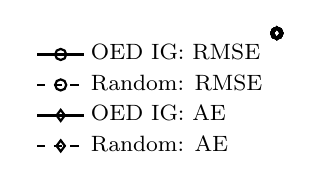
\begin{tikzpicture}

\begin{axis}[%
width=0.951\fwidth,
height=\hwidth,
at={(0\fwidth,0\hwidth)},
scale only axis,
unbounded coords=jump,
xmin=0.75,
xmax=4.25,
xtick={1,2,3,4},
xticklabels={{72},{168},{240},{336}},
xlabel style={font=\color{white!15!black}},
xlabel={no of hours},
ymin=10,
ymax=65,
ylabel style={font=\color{white!15!black}},
ylabel={error [kW]},
axis background/.style={fill=white},
legend style={legend cell align=left, align=left, fill=none, draw=none},
xlabel style={font=\footnotesize},ylabel style={font=\footnotesize},legend style={font=\footnotesize},ticklabel style={font=\footnotesize},ylabel shift = -5 pt,xlabel shift = -5 pt,
]
\addplot [color=black, line width=0.8pt, mark=o, mark options={solid, black}]
  table[row sep=crcr]{%
1	38.3577768196538\\
2	23.5762131941091\\
3	22.2379994094524\\
4	22.0269257238242\\
5	nan\\
};
\addlegendentry{OED IG: RMSE}

\addplot [color=black, dashed, line width=0.8pt, mark=o, mark options={solid, black}]
  table[row sep=crcr]{%
1	60.5953168967942\\
2	33.7867759715775\\
3	25.1122218421038\\
4	23.931187395704\\
5	nan\\
};
\addlegendentry{Random: RMSE}

\addplot [color=black, line width=0.8pt, mark=diamond, mark options={solid, black}]
  table[row sep=crcr]{%
1	29.3576068831179\\
2	17.6386666958257\\
3	16.0967115004186\\
4	15.9556477539858\\
5	nan\\
};
\addlegendentry{OED IG: AE}

\addplot [color=black, dashed, line width=0.8pt, mark=diamond, mark options={solid, black}]
  table[row sep=crcr]{%
1	46.4640980105609\\
2	25.1777970816288\\
3	18.7235731225753\\
4	17.3664780029757\\
5	nan\\
};
\addlegendentry{Random: AE}

\end{axis}
\end{tikzpicture}%
  \caption{Error in prediction of power consumption on test dataset. RMSE denotes root mean square error and AE denotes absolute error. The errors are much lower with optimal experiment design based on information gain. The random sampling requires \(2 \times\) time to reach the same accuracy as OED.}
  % \captionsetup{justification=centering}
  \vspace{-12pt}
  \label{F:oed:example}
\end{figure}

%%% Local Variables:
%%% mode: latex
%%% TeX-master: "main"
%%% End:


\section{Learning-based Control Smart Energy Systems}
\label{sec:control}
\begin{todo}
  Using GP in MPC. Briefly present various applications (as in BPACS paper).
\end{todo}

Using these measurement data, we learn autoregressive GP models \(\mathcal{M}_1\) and \(\mathcal{M}_2\), and use the zero-variance method to predict the future output \(y_{t+\tau}\), where $t$ is the current time and \( \tau \ge 0\).
Specifically,
\begin{gather}
\label{eq:dpc:prediction}
y_{t+\tau} \sim \GaussianDist{\bar{y}_{t+\tau} = g_{\mathrm m}(x_{t+\tau})}{\sigma^2_{y, t+\tau} = g_{\mathrm v}(x_{t+\tau})}, \\
x_{t + \tau} = [\bar y_{t+ \tau-l}, \dots, \bar y_{t+ \tau-1}, u_{t+ \tau-m}, \dots, u_{t+ \tau}, \nonumber \\
\qquad\qquad\qquad\qquad  w_{t+ \tau-p}, \dots, w_{t+ \tau-1}, w_{t+ \tau}]\text, \nonumber
\end{gather}
in which \(w:=[d^w, d^p]\).
It is assumed that at time \(t\), \(w_{t+\tau}\) are available \(\forall \tau \) from forecasts or fixed rules as applicable.
For the GP, we use a constant mean function and the special covariance function proposed in our previous work \cite{nghiemetal16gp} to capture both the temporal pattern of the energy usage and the effect of non-temporal features, such as weather conditions and temperature setpoints, on the power demand.
We optimize the hyperparameters \(\theta\) % = [\mu, k, \sigma_{f_2}, \lambda_d, \sigma_{f_3}, \alpha, \lambda] \)
of the GP model using GPML \cite{Rasmussen2010}.


In a multistep simulation of a dynamical GP, the autoregressive outputs fed to the model beyond the first step are random variables, resulting in more and more complex output distributions as we go further.
Therefore, it involves uncertainty propagation through the model, which would complicate the computation of the model significantly.
\cite{nghiemetal16gp} showed that a simple simulation method called \emph{zero-variance method}, which replaces the autoregressive signals with their corresponding expected values, could achieve sufficient prediction accuracy while benefitting from computational simplicity.
In this paper, the zero-variance method was selected for predicting future outputs in optimization formulations.


%%% Local Variables:
%%% mode: latex
%%% TeX-master: "main"
%%% End:


\section{Learning to Adapt Smart Energy Systems}
\label{sec:adapt}

%%% Local Variables:
%%% mode: latex
%%% TeX-master: "main"
%%% End:


\section{Implementation and Case Study}
\label{sec:case-study}
\begin{todo}
  The ICONICS implementation, dashboard, Achin's implementation with Tensorflow on ACS (just an overview, no need to reveal details).
  A brief case study.
\end{todo}


%%% Local Variables:
%%% mode: latex
%%% TeX-master: "main"
%%% End:


\section{Conclusion}
\label{sec:conclusion}

%%% Local Variables:
%%% mode: latex
%%% TeX-master: "main"
%%% End:


% if have a single appendix:
%\appendix[Proof of the Zonklar Equations]
% or
%\appendix  % for no appendix heading
% do not use \section anymore after \appendix, only \section*
% is possibly needed

% use appendices with more than one appendix
% then use \section to start each appendix
% you must declare a \section before using any
% \subsection or using \label (\appendices by itself
% starts a section numbered zero.)
%


\appendices
% \section{Appendix}

% you can choose not to have a title for an appendix
% if you want by leaving the argument blank
% \section{}


% use section* for acknowledgment
\section*{Acknowledgment}


The authors would like to thank...


% Can use something like this to put references on a page
% by themselves when using endfloat and the captionsoff option.
\ifCLASSOPTIONcaptionsoff
  \newpage
\fi



% trigger a \newpage just before the given reference
% number - used to balance the columns on the last page
% adjust value as needed - may need to be readjusted if
% the document is modified later
%\IEEEtriggeratref{8}
% The "triggered" command can be changed if desired:
%\IEEEtriggercmd{\enlargethispage{-5in}}

% references section

% can use a bibliography generated by BibTeX as a .bbl file
% BibTeX documentation can be easily obtained at:
% http://mirror.ctan.org/biblio/bibtex/contrib/doc/
% The IEEEtran BibTeX style support page is at:
% http://www.michaelshell.org/tex/ieeetran/bibtex/
\bibliographystyle{IEEEtran}
% argument is your BibTeX string definitions and bibliography database(s)
\bibliography{references}
%
% <OR> manually copy in the resultant .bbl file
% set second argument of \begin to the number of references
% (used to reserve space for the reference number labels box)
% \begin{thebibliography}{99}
% \end{thebibliography}

% biography section
% 
% If you have an EPS/PDF photo (graphicx package needed) extra braces are
% needed around the contents of the optional argument to biography to prevent
% the LaTeX parser from getting confused when it sees the complicated
% \includegraphics command within an optional argument. (You could create
% your own custom macro containing the \includegraphics command to make things
% simpler here.)
%\begin{IEEEbiography}[{\includegraphics[width=1in,height=1.25in,clip,keepaspectratio]{mshell}}]{Michael Shell}
% or if you just want to reserve a space for a photo:

% \begin{IEEEbiography}{Truong X. Nghiem}
% \end{IEEEbiography}

% if you will not have a photo at all:
% \begin{IEEEbiography}{Achin Jain}
% \end{IEEEbiography}

% insert where needed to balance the two columns on the last page with
% biographies
%\newpage

% \begin{IEEEbiography}{Rahul Mangharam}
% \end{IEEEbiography}

% You can push biographies down or up by placing
% a \vfill before or after them. The appropriate
% use of \vfill depends on what kind of text is
% on the last page and whether or not the columns
% are being equalized.

%\vfill

% Can be used to pull up biographies so that the bottom of the last one
% is flush with the other column.
%\enlargethispage{-5in}



% that's all folks
\end{document}



%%% Local Variables:
%%% mode: latex
%%% TeX-master: t
%%% End:
